
\begin{frame}{The Faust Ecosystem}{Compilers}
	
\begin{itemize}
\item Command Line Compilers
	\begin{itemize}
	\item \lstinline'faust' command line
	\item \lstinline'faust2xxx' command line
	\item FaustWorks (IDE)
	\end{itemize}
\item Embedded Compilers (libfaust with the LLVM backend)
	\begin{itemize}
	\item FaustLive (self contained)
	\item Faustgen for Max/MSP
	\item Faustcompile, etc. for Csound (V. Lazzarini)
	\item Faust4processing
	\item Antescofo (IRCAM's score follower)
	\end{itemize}
\item Web Based Compilers
	\begin{itemize}
	\item Online documentation (\url{https://faustdoc.grame.fr})
	\item Faustplayground (\url{https://faustplayground.grame.fr})
	\item Online IDE (\url{https://faustide.grame.fr})
	\end{itemize}

\end{itemize}
\end{frame}

\begin{frame}{The Faust Ecosystem}{Libraries}

\begin{itemize}
\item The Faust libraries implement hundreds of DSP functions for audio processing and synthesis. They are organized by types in a set of .lib files (e.g., envelopes.lib, filters.lib, etc.).
\item All documented at: \url{https://faustlibraries.grame.fr}
\item And community contributions here: \url{https://faustlibraries.grame.fr/community}
\end{itemize}

\end{frame}

\begin{frame}[fragile]{The Faust Ecosystem}
	\centering
	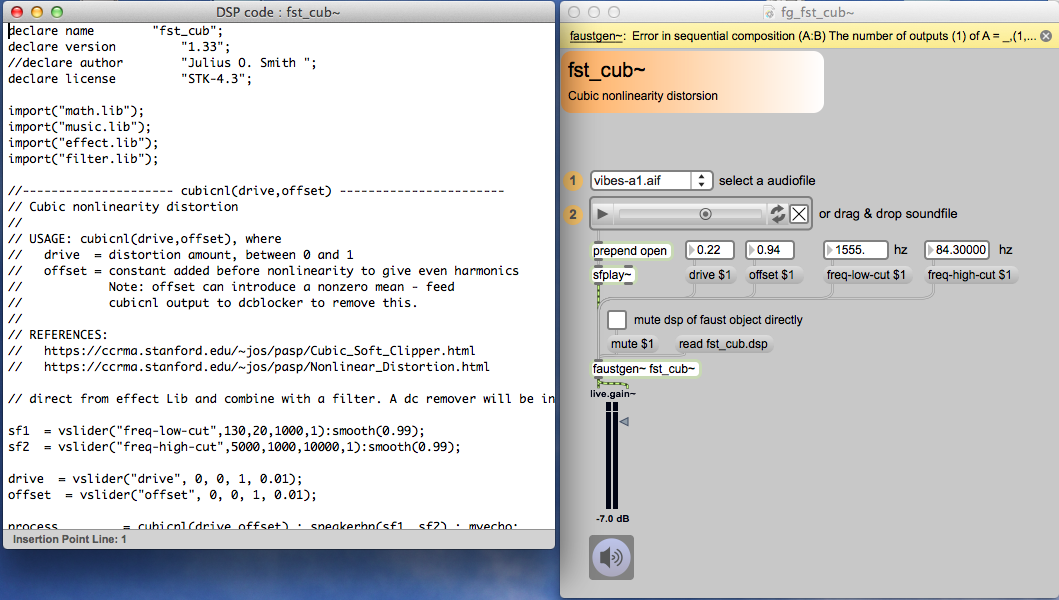
\includegraphics[width=0.45\textwidth]{images/faustgen}
	\hspace{0.25cm}
	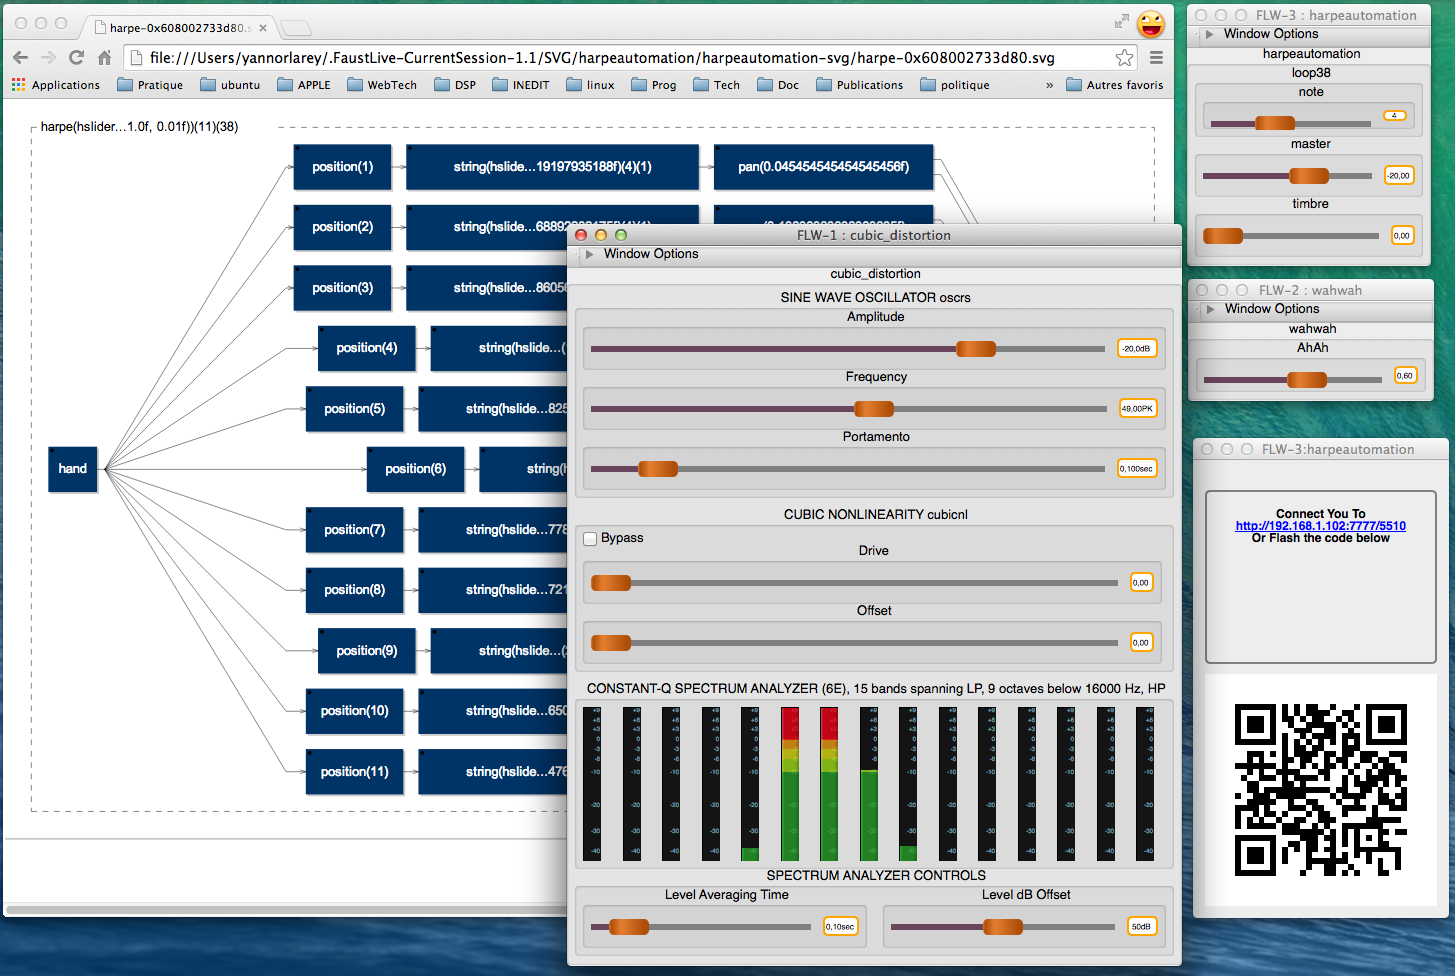
\includegraphics[width=0.36\textwidth]{images/FaustLiveSession}
	\vspace{0.25cm}
	\href{https://faustplayground.grame.fr/}{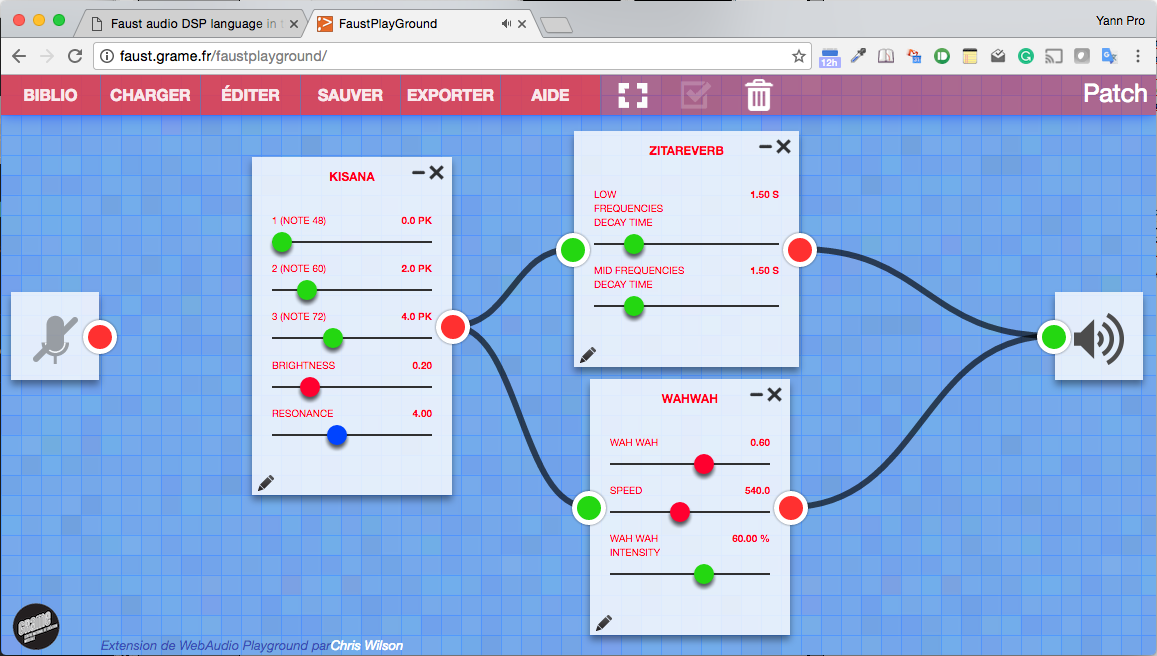
\includegraphics[width=0.45\textwidth]{images/faustplayground1}}
	\hspace{0.1cm}
	\href{https://fausteditor.grame.fr/}{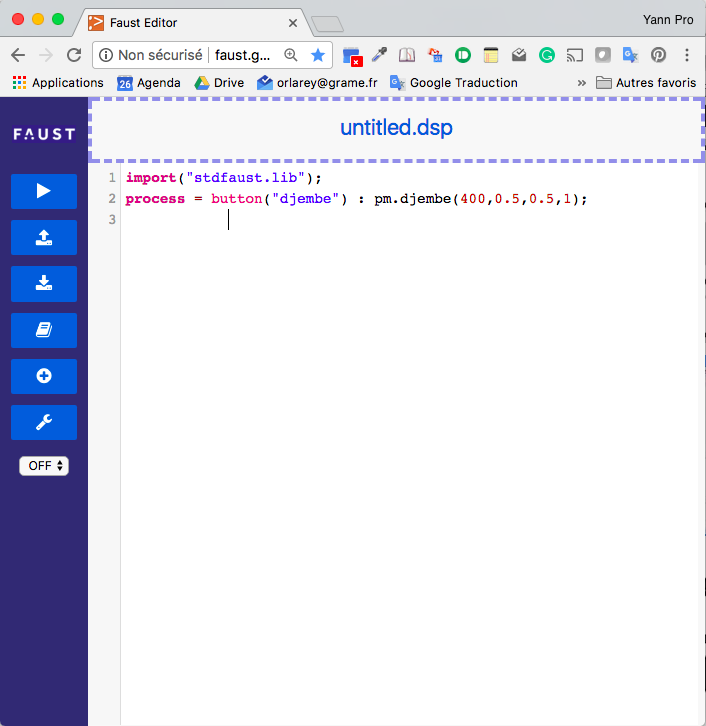
\includegraphics[width=0.25\textwidth]{images/faust-editor.png}}
	\hspace{0.1cm}
	\href{https://faustide.grame.fr/}{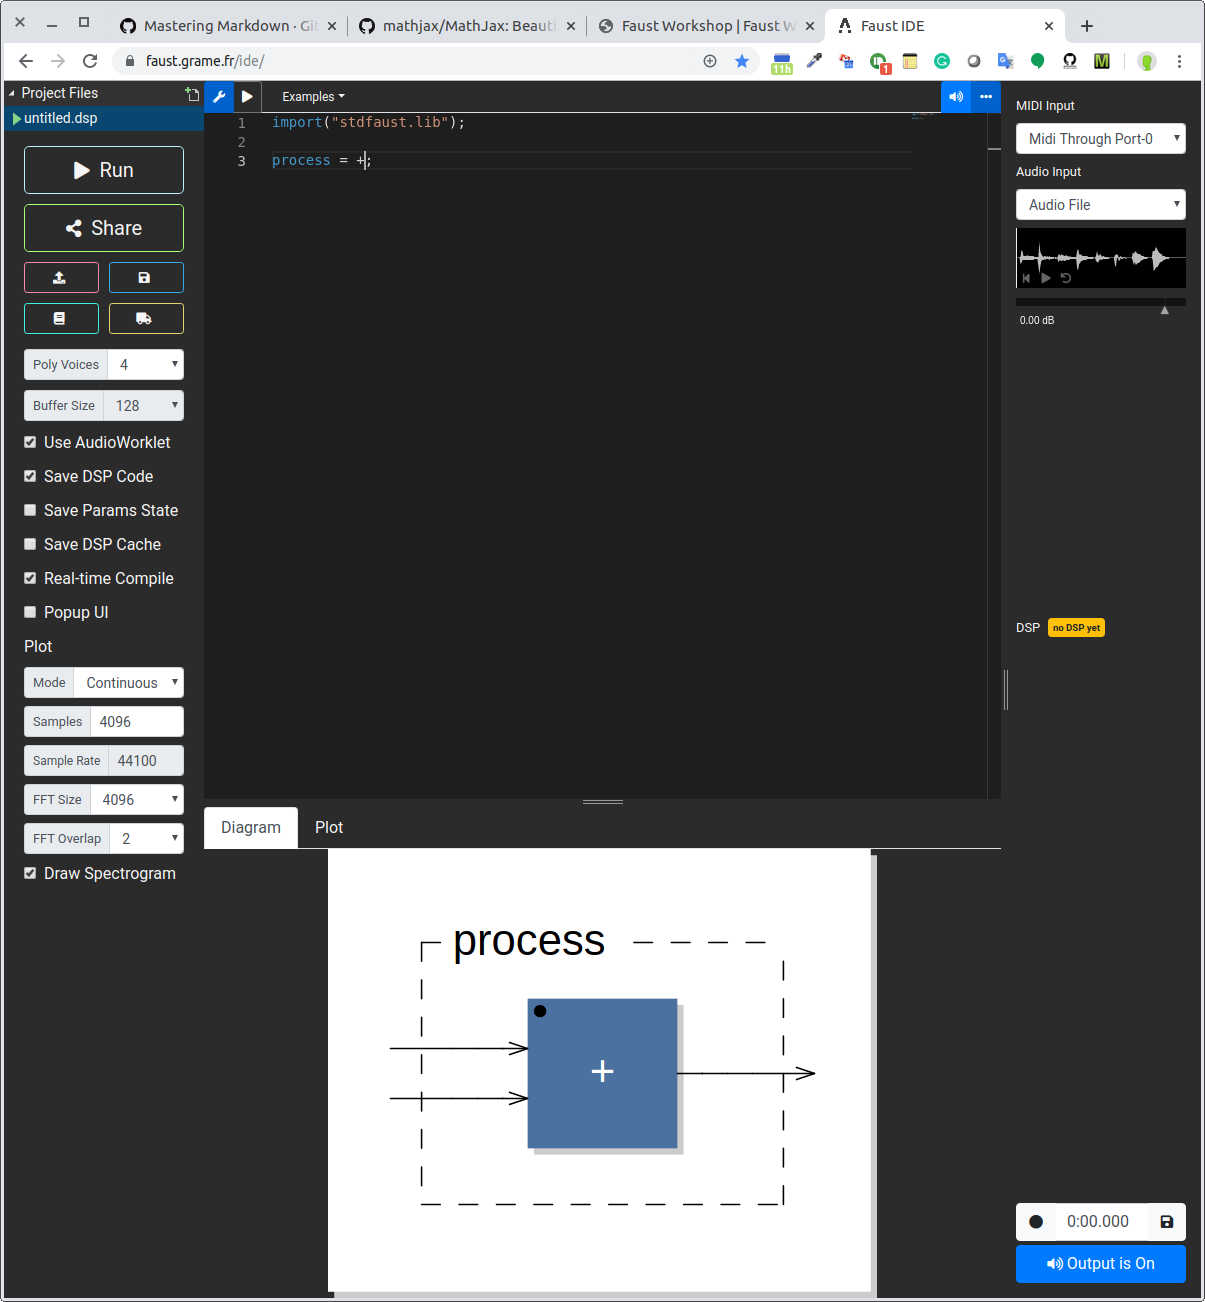
\includegraphics[width=0.23\textwidth]{images/faust-ide.png}}
\end{frame}
